\begin{frame}
	\frametitle{Git Object Hashmap}

	\begin{columns}
	\begin{column}{0.5\textwidth}
		\begin{itemize}
			\item blob
			\item tree
			\item commit
			\item tag (or are they?)
		\end{itemize}
	\end{column}
	\begin{column}{0.5\textwidth}
		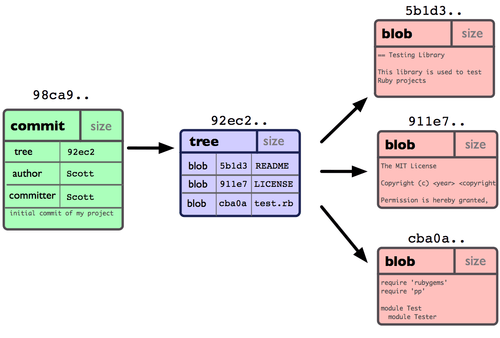
\includegraphics[width=\textwidth]{images/object-types.png}
	\end{column}
	\end{columns}

	\note[itemize]{
		\item all these are compressed
		\item have a tag at the top that tells git what the type is.
		\item blob is flat file copy
	}
\end{frame}

\begin{frame}[fragile]
	\frametitle{blob}

	\begin{columns}
	\begin{column}{0.5\textwidth}
		\begin{itemize}
		\item flat files
		\item the actual source code
		\item full copy
		\item has no further references to other objects
		\end{itemize}
	\end{column}
	\begin{column}{0.5\textwidth}
		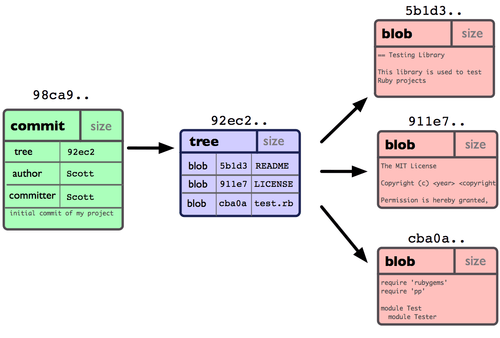
\includegraphics[width=\textwidth]{images/object-types.png}
	\end{column}
	\end{columns}

	\note[itemize]{
		\item blob is flat file copy
	}
\end{frame}

\begin{frame}[fragile]
	\frametitle{tree}

	\begin{columns}
	\begin{column}{0.5\textwidth}
		\begin{itemize}
		\item represents a directory on disk
		\item retains file permissions (in unix notation)
		\item points to other trees and blobs
		\end{itemize}
	\end{column}
	\begin{column}{0.5\textwidth}
		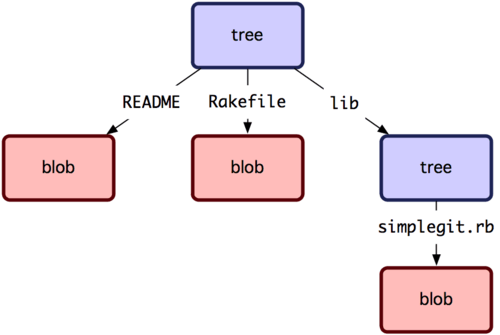
\includegraphics[width=\textwidth]{images/trees.png}
	\end{column}
	\end{columns}

\end{frame}

\begin{frame}[fragile]
	\frametitle{commit}

	\begin{columns}
	\begin{column}{0.5\textwidth}
		\begin{itemize}
		\item stores author, timestamp, message, ...
		\item points to a tree
		\item points to 1 or more commits (parent commits)
		\end{itemize}
	\end{column}
	\begin{column}{0.5\textwidth}
		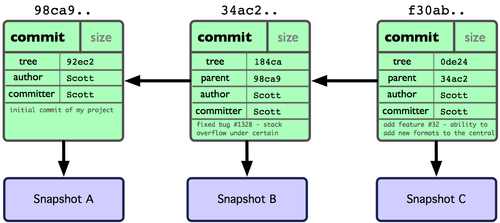
\includegraphics[width=\textwidth]{images/commits.png}
	\end{column}
	\end{columns}

	\note[itemize]{
		\item history is represented solely in commit objects, it has noting to do with
		code, trees, or blobs.
	}
\end{frame}

\begin{frame}
	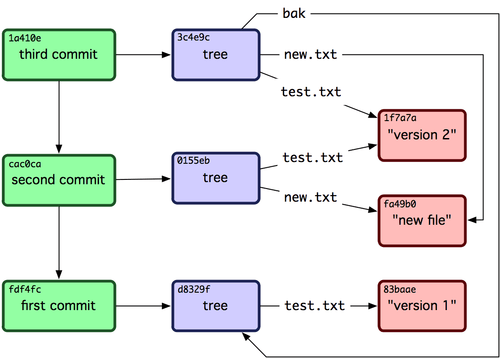
\includegraphics[width=\textwidth]{images/git-objects.png}
\end{frame}
